\documentclass{beamer}
\usepackage{tikz}
\usepackage{amsmath}

\usetheme{Madrid}
\usecolortheme{seahorse}

\title{Statistical Reasoning: From Samples to Populations}
\author{Brendan Shea, PhD}
\date{Introduction to Logic}

\begin{document}
	
	\frame{\titlepage}
	
	% Slide 1: Title Slide
	\begin{frame}
		\frametitle{Statistical Reasoning: From Samples to Populations}
		\begin{center}
			{\Large Welcome to the World of Statistical Thinking}
		\end{center}
		
		\begin{itemize}
			\item Today we'll explore how we can learn about large groups by studying smaller parts of them.
			\item We'll discover why opinion polls can predict elections and how scientific studies reveal truths about the world.
			\item You'll learn to spot good reasoning from bad reasoning when people make claims based on data.
			\item By the end, you'll have the tools to be a smart consumer of statistics in everyday life.
		\end{itemize}
		
		\begin{block}{Course Goal}
			To understand how \textbf{inductive reasoning} works with data and samples to help us make informed decisions about populations and the world around us.
		\end{block}
		
	\end{frame}
	
	% Slide 2: What is Statistical Reasoning?
	\begin{frame}
		\frametitle{What is Statistical Reasoning?}
		
		\begin{itemize}
			\item \textbf{Statistical reasoning} is the process of using data from a small group to make educated guesses about a larger group.
			\item It's a special type of thinking that helps us move from specific observations to general conclusions.
			\item Unlike mathematical proofs, statistical reasoning deals with uncertainty and probability rather than absolute certainty.
			\item This type of reasoning is everywhere: from medical research to business decisions to political polling.
		\end{itemize}
		
		\begin{example}
			If we survey 1,000 randomly chosen citizens of Gotham City about their favorite superhero, we can use their answers to estimate what all 2 million Gotham citizens think—even though we didn't ask everyone!
		\end{example}
		
	\end{frame}
	
	% Slide 3: Why Statistical Reasoning Matters
	\begin{frame}
		\frametitle{Why Statistical Reasoning Matters}
		
		\begin{itemize}
			\item Every day you encounter claims based on statistical reasoning: ``9 out of 10 doctors recommend...'' or ``New study shows...''
			\item Understanding these concepts helps you separate reliable information from misleading or false claims.
			\item Good statistical reasoning skills protect you from being fooled by biased surveys, cherry-picked data, or poorly designed studies.
			\item These skills are essential for making informed decisions about health, politics, finances, and other important life choices.
		\end{itemize}
		
		\begin{alertblock}{Real-World Impact}
			Poor statistical reasoning can lead to bad medical decisions, wasted money on ineffective products, or voting based on misleading poll information. Learning these skills literally improves your life!
		\end{alertblock}
		
	\end{frame}
	
	% Slide 4: Inductive vs. Deductive Reasoning
	\begin{frame}
		\frametitle{Inductive vs. Deductive Reasoning}
		
		\begin{itemize}
			\item \textbf{Deductive reasoning} claims that the conclusion necessarily follows from the premises—if the premises are true, the conclusion must be true.
			\item \textbf{Inductive reasoning} claims that the conclusion probably follows from the premises—the evidence makes the conclusion likely but not guaranteed.
			\item Statistical reasoning is a form of inductive reasoning because we use sample data to make probable claims about populations.
			\item The strength of inductive reasoning depends on the quality and quantity of our evidence.
		\end{itemize}
		
\begin{center}
	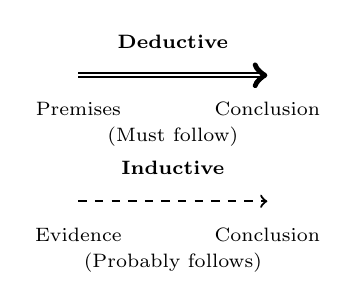
\begin{tikzpicture}[scale=0.8]
		\scriptsize
		% Deductive - strong connection
		\draw[thick, double, ->] (0,2) -- (3,2);
		\node[above] at (1.5,2.3) {\textbf{Deductive}};
		\node[below] at (0,1.7) {Premises};
		\node[below] at (3,1.7) {Conclusion};
		\node[below] at (1.5,1.3) {(Must follow)};
		
		% Inductive - weaker connection
		\draw[thick, dashed, ->] (0,0) -- (3,0);
		\node[above] at (1.5,0.3) {\textbf{Inductive}};
		\node[below] at (0,-0.3) {Evidence};
		\node[below] at (3,-0.3) {Conclusion};
		\node[below] at (1.5,-0.7) {(Probably follows)};
	\end{tikzpicture}
\end{center}
		
	\end{frame}
	
	% Slides 5-8: Foundations
	
	% Slide 5: Populations vs. Samples
	\begin{frame}
		\frametitle{Populations vs. Samples}
		
		\begin{itemize}
			\item A \textbf{population} is the entire group of individuals or items that we want to learn about or make conclusions about.
			\item A \textbf{sample} is a smaller subset of the population that we actually observe, measure, or survey.
			\item We study samples because it's usually impossible, too expensive, or too time-consuming to study every member of a population.
			\item The goal is to use information from our sample to make accurate inferences about the entire population.
		\end{itemize}
		
		\begin{center}
			\begin{tabular}{|l|l|l|}
				\hline
				\textbf{Scenario} & \textbf{Population} & \textbf{Sample} \\
				\hline
				Springfield Election & All registered voters & 800 voters polled \\
				\hline
				Emerald City Health & All city residents & 1,200 people surveyed \\
				\hline
				Gotham Crime Study & All reported crimes & 500 cases reviewed \\
				\hline
			\end{tabular}
		\end{center}
		
	\end{frame}
	
	% Slide 6: The Challenge of Making Generalizations
	\begin{frame}
		\frametitle{The Challenge of Making Generalizations}
		
		\begin{itemize}
			\item When we generalize from a sample to a population, we're making an \textbf{inductive leap}—going beyond what we directly observed.
			\item This leap involves uncertainty because we haven't examined every member of the population.
			\item The challenge is to make this leap as safely and accurately as possible by using good sampling methods.
			\item Even with perfect methods, there's always some chance that our sample doesn't perfectly represent the population.
		\end{itemize}
		
		\begin{alertblock}{The Fundamental Challenge}
			How can we be confident that what we observe in our sample actually reflects what's true in the larger population? This is the central question of statistical reasoning.
		\end{alertblock}
		
	\end{frame}
	
	% Slide 7: What Makes a Good Sample?
	\begin{frame}
		\frametitle{What Makes a Good Sample?}
		
		\begin{itemize}
			\item A good sample should be \textbf{representative}—it should accurately reflect the characteristics of the population.
			\item The sample should be large enough to capture the diversity within the population, but size alone doesn't guarantee quality.
			\item \textbf{Random selection} is crucial because it gives every member of the population an equal chance of being included.
			\item The sample should be free from systematic bias that might skew the results in one direction.
		\end{itemize}
		
		\begin{block}{Key Principles of Good Sampling}
			\begin{itemize}
				\item \textbf{Randomness}: Every population member has an equal chance of selection
				\item \textbf{Representativeness}: Sample reflects population diversity
				\item \textbf{Adequate size}: Large enough to capture important patterns
				\item \textbf{Bias-free}: No systematic exclusions or distortions
			\end{itemize}
		\end{block}
		
	\end{frame}
	
	% Slide 8: Common Sampling Mistakes
	\begin{frame}
		\frametitle{Common Sampling Mistakes}
		
		\begin{itemize}
			\item \textbf{Convenience sampling} occurs when researchers choose the easiest people to survey rather than a random selection.
			\item \textbf{Voluntary response bias} happens when only people with strong opinions choose to participate in a survey.
			\item \textbf{Undercoverage} occurs when some groups in the population have no chance of being selected for the sample.
			\item \textbf{Non-response bias} happens when certain types of people systematically refuse to participate in the study.
		\end{itemize}
		
		\begin{example}
			A radio station asks listeners to call in with their opinion on a new tax proposal. This suffers from voluntary response bias (only motivated people call) and undercoverage (only radio listeners can participate). The results won't represent the general population's views.
		\end{example}
		
	\end{frame}
	% Slides 9-12: Sampling Methods Part 1
	
	% Slide 9: Random Sampling: The Gold Standard
	\begin{frame}
		\frametitle{Random Sampling: The Gold Standard}
		
		\begin{itemize}
			\item \textbf{Random sampling} means every member of the population has an equal probability of being selected for the sample.
			\item This method eliminates human bias in choosing who gets included and who gets left out of the study.
			\item Random sampling doesn't guarantee a perfect sample, but it gives us the best chance of getting a representative one.
			\item It also allows us to calculate how confident we can be in our results using mathematical formulas.
		\end{itemize}
		
		\begin{block}{Why Random Sampling Works}
			When selection is truly random, any biases in the population tend to cancel each other out in the sample. Over many random samples, the average result will be very close to the true population value.
		\end{block}
		
	\end{frame}
	
	% Slide 10: Simple Random Sampling in Research
	\begin{frame}
		\frametitle{Simple Random Sampling in Research}
		
		\begin{itemize}
			\item \textbf{Simple random sampling} gives every possible group of the same size an equal chance of being selected.
			\item Medical researchers might randomly select 1,000 patients from a hospital database to study the effectiveness of a new treatment.
			\item Educational researchers could randomly choose 500 students from all students in a school district to study learning outcomes.
			\item This ensures that different types of people (young/old, rich/poor, healthy/sick) all have equal chances of being included.
		\end{itemize}
		
		\begin{exampleblock}{Example}
			The Gotham City Health Department wants to study diabetes rates among adults. They have a database of all 1.5 million adult residents. A computer randomly generates 2,000 ID numbers, and those people are contacted for health screenings. This simple random sampling ensures the study includes people from all neighborhoods, income levels, and age groups.
		\end{exampleblock}
		
	\end{frame}
	
	% Slide 11: Systematic Sampling
	\begin{frame}
		\frametitle{Systematic Sampling}
		
		\begin{itemize}
			\item \textbf{Systematic sampling} involves selecting every nth person from a list, where n is calculated by dividing population size by desired sample size.
			\item This method is easier to implement than simple random sampling when you have a complete list of the population.
			\item It works well when the list is in random order, but can introduce bias if there's a pattern in how the list is organized.
			\item The first person selected should be chosen randomly, then every nth person after that.
		\end{itemize}
		
		\begin{center}
			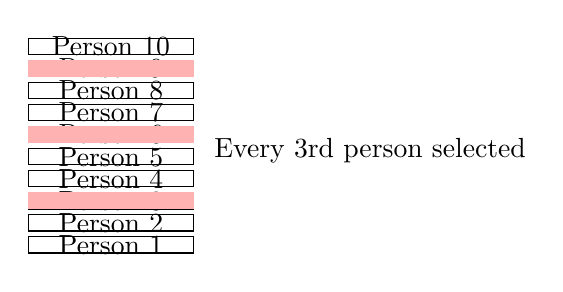
\begin{tikzpicture}[scale=0.7]
				% Draw a list representation
				\foreach \i in {1,...,10} {
					\draw (0,\i*0.4) rectangle (3,\i*0.4+0.3);
					\node at (1.5,\i*0.4+0.15) {Person \i};
				}
				% Highlight every 3rd person
				\fill[red!30] (0,1.2) rectangle (3,1.5);
				\fill[red!30] (0,2.4) rectangle (3,2.7);
				\fill[red!30] (0,3.6) rectangle (3,3.9);
				\node[right] at (3.2,2.25) {Every 3rd person selected};
			\end{tikzpicture}
		\end{center}
		
	\end{frame}
	
	% Slide 12: Stratified Sampling in Educational Research
	\begin{frame}
		\frametitle{Stratified Sampling in Educational Research}
		
		\begin{itemize}
			\item \textbf{Stratified sampling} divides the population into subgroups (strata) based on important characteristics, then randomly samples from each stratum.
			\item This ensures that important subgroups are properly represented in the final sample.
			\item It's especially useful when some groups are much smaller than others in the population.
			\item Each stratum should be internally similar but different from other strata on the characteristic of interest.
		\end{itemize}
		
		\begin{exampleblock}{Example}
			Researchers want to study reading achievement across Springfield's school district. They divide schools into strata: Elementary (40\%), Middle (30\%), and High School (30\%). Instead of hoping random sampling captures this mix, they deliberately sample 400 elementary students, 300 middle school students, and 300 high school students for a total sample of 1,000.
		\end{exampleblock}
		
	\end{frame}	
	
	% Slides 13-16: Sampling Methods Part 2 and Sample Size
	
	% Slide 13: Cluster Sampling
	\begin{frame}
		\frametitle{Cluster Sampling}
		
		\begin{itemize}
			\item \textbf{Cluster sampling} divides the population into groups (clusters), randomly selects some clusters, then surveys everyone within the chosen clusters.
			\item This method is useful when it's difficult or expensive to travel to many different locations.
			\item Clusters should ideally be mini-versions of the entire population, containing similar diversity.
			\item It's less precise than other methods but much more practical and cost-effective for large geographic areas.
		\end{itemize}
		
		\begin{block}{Cluster Sampling Process}
			\begin{enumerate}
				\item Divide population into clusters (e.g., city blocks, schools, hospitals)
				\item Randomly select a subset of clusters
				\item Survey all individuals within the selected clusters
				\item Combine results to make inferences about the entire population
			\end{enumerate}
		\end{block}
		
	\end{frame}
	
	% Slide 14: Convenience Sampling: Why It's Problematic
	\begin{frame}
		\frametitle{Convenience Sampling: Why It's Problematic}
		
		\begin{itemize}
			\item \textbf{Convenience sampling} involves choosing the easiest people to survey—those who are readily available or accessible.
			\item This method seems efficient but often produces biased results because certain groups are systematically excluded.
			\item People who are easily accessible often share similar characteristics that don't represent the broader population.
			\item While convenient and cheap, this method severely limits our ability to generalize findings to the larger population.
		\end{itemize}
		
		\begin{alertblock}{Why Convenience Sampling Fails}
			A college student surveying people at a shopping mall on Tuesday afternoon will miss working people, students in class, people without transportation, and many others. The sample will be biased toward people with flexible schedules and disposable income.
		\end{alertblock}
		
	\end{frame}
	
	% Slide 15: Bias in Sampling: The Emerald City Election Poll
	\begin{frame}
		\frametitle{Bias in Sampling: The Emerald City Election Poll}
		
		\begin{itemize}
			\item \textbf{Sampling bias} occurs when the sample systematically differs from the population in ways that affect the results.
			\item This bias can happen even with large samples if the selection method is flawed.
			\item Bias can be introduced through the sampling frame (the list we sample from), the selection method, or non-response patterns.
			\item Once bias is introduced, increasing sample size won't fix the problem—it just gives us more precise wrong answers.
		\end{itemize}
		
		\begin{example}
			The Emerald City Tribune wants to predict the mayoral election. They survey 10,000 people by calling landline phone numbers during business hours. This introduces bias: they miss people without landlines (often younger/poorer), people at work, and people who don't answer unknown numbers. Despite the large sample, results may not reflect actual voter preferences.
		\end{example}
		
	\end{frame}
	
	% Slide 16: Does Sample Size Matter?
	\begin{frame}
		\frametitle{Does Sample Size Matter?}
		
		\begin{itemize}
			\item Sample size does matter, but it's not the only factor that determines the quality of statistical reasoning.
			\item Larger samples generally give more precise estimates and reduce the role of random variation.
			\item However, a large biased sample is worse than a smaller unbiased sample for making accurate inferences.
			\item The relationship between sample size and accuracy follows the \textbf{law of diminishing returns}—doubling the sample size doesn't double the accuracy.
		\end{itemize}
		
		\begin{center}
			\begin{tabular}{|c|c|c|}
				\hline
				\textbf{Sample Size} & \textbf{Margin of Error} & \textbf{Cost to Improve} \\
				\hline
				100 & ±10\% & Low \\
				\hline
				400 & ±5\% & Medium \\
				\hline
				1,600 & ±2.5\% & High \\
				\hline
				6,400 & ±1.25\% & Very High \\
				\hline
			\end{tabular}
		\end{center}
		
	\end{frame}
	% Slides 17-20: Sample Size and Representation
	
	% Slide 17: The Law of Large Numbers (Simple Version)
	\begin{frame}
		\frametitle{The Law of Large Numbers (Simple Version)}
		
		\begin{itemize}
			\item The \textbf{Law of Large Numbers} states that as sample size increases, sample results get closer to the true population value.
			\item This law explains why larger samples are generally more reliable than smaller ones for estimating population characteristics.
			\item However, the improvement in accuracy slows down as samples get larger—you need four times as many people to cut the margin of error in half.
			\item This law only works when sampling is done properly; it cannot fix bias or poor sampling methods.
		\end{itemize}
		
		\begin{center}
			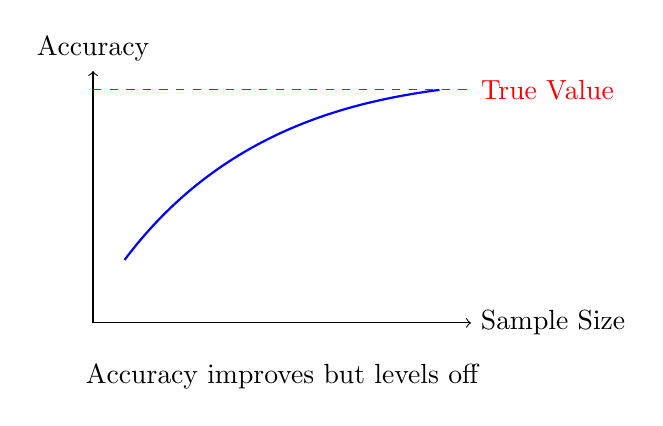
\begin{tikzpicture}[scale=0.8]
				\draw[->] (0,0) -- (6,0) node[right] {Sample Size};
				\draw[->] (0,0) -- (0,4) node[above] {Accuracy};
				\draw[thick, blue] (0.5,1) .. controls (2,3) and (4,3.5) .. (5.5,3.7);
				\node[below] at (3,-0.5) {Accuracy improves but levels off};
				\draw[dashed, red] (0,3.7) -- (6,3.7) node[right] {True Value};
			\end{tikzpicture}
		\end{center}
		
	\end{frame}
	
	% Slide 18: When Small Samples Can Mislead
	\begin{frame}
		\frametitle{When Small Samples Can Mislead}
		
		\begin{itemize}
			\item Small samples are more susceptible to random variation and may not capture the diversity within a population.
			\item Unusual or extreme cases have a bigger impact on small samples, potentially leading to misleading conclusions.
			\item Small samples may miss important subgroups entirely, especially minorities or people with rare characteristics.
			\item While small samples can suggest interesting patterns, we should be cautious about making strong claims based on limited data.
		\end{itemize}
		
		\begin{example}
			A researcher surveys 20 Gotham City residents about crime concerns and finds that 90\% are worried about street crime. However, by chance, 18 of the 20 people lived in high-crime neighborhoods. A larger sample of 500 people shows only 45\% are worried about street crime, revealing that the small sample was misleading.
		\end{example}
		
	\end{frame}
	
	% Slide 19: Diminishing Returns: Why Bigger Isn't Always Better
	\begin{frame}
		\frametitle{Diminishing Returns: Why Bigger Isn't Always Better}
		
		\begin{itemize}
			\item The improvement in accuracy from increasing sample size follows a pattern of \textbf{diminishing returns}.
			\item Going from 100 to 400 people gives a big improvement, but going from 1,000 to 4,000 people gives a much smaller improvement.
			\item At some point, the cost and effort of a larger sample outweigh the small gain in accuracy.
			\item Most professional polls use samples of 1,000-1,500 people because this provides a good balance of accuracy and cost.
		\end{itemize}
		
		\begin{block}{The Square Root Rule}
			To cut your margin of error in half, you need to quadruple your sample size. This means the cost of improvement grows very quickly:
			\begin{itemize}
				\item 100 → 400 people: Error cuts from 10\% to 5\%
				\item 400 → 1,600 people: Error cuts from 5\% to 2.5\%
				\item 1,600 → 6,400 people: Error cuts from 2.5\% to 1.25\%
			\end{itemize}
		\end{block}
		
	\end{frame}
	
	% Slide 20: Representative Samples vs. Large Samples
	\begin{frame}
		\frametitle{Representative Samples vs. Large Samples}
		
		\begin{itemize}
			\item A \textbf{representative sample} accurately reflects the characteristics of the population, regardless of size.
			\item A representative sample of 1,000 people is much better than a biased sample of 10,000 people for making accurate inferences.
			\item The goal is to get the most representative sample possible within your budget and time constraints.
			\item Quality of sampling method matters more than quantity when it comes to making reliable generalizations.
		\end{itemize}
		
		\begin{alertblock}{Quality vs. Quantity}
			The 1936 Literary Digest poll surveyed 2.4 million people and predicted that Alf Landon would defeat Franklin Roosevelt by a landslide. Roosevelt actually won by a landslide! The massive sample was biased toward wealthy people who could afford cars and telephones. A smaller but representative sample would have been far more accurate.
		\end{alertblock}
		
		\end{frame}

% Slides 21-24: Understanding Studies and Informal Reasoning

% Slide 21: Anatomy of a Research Study
\begin{frame}
	\frametitle{Anatomy of a Research Study}
	
	\begin{itemize}
		\item A good research study reports several key pieces of information: the research question, who was studied, how data was collected, and what the results mean.
		\item The \textbf{sampling method} tells you how participants were chosen and helps you judge if the sample represents the target population.
		\item The \textbf{methodology} describes exactly how measurements were taken, which affects the reliability of the conclusions.
		\item \textbf{Context} matters enormously—when and where the study was conducted can influence how broadly we can apply the results.
	\end{itemize}
	
	\begin{block}{Essential Study Information}
		\scriptsize
		\begin{itemize}
			\item \textbf{Who}: Which population was studied (patients, students, consumers, etc.)
			\item \textbf{When \& Where}: Time period and location of the research
			\item \textbf{How}: Method used (survey, experiment, observation)
			\item \textbf{Sample size}: Number of people or cases studied
			\item \textbf{Limitations}: What the researchers acknowledge they cannot conclude
		\end{itemize}
	\end{block}
	
\end{frame}

% Slide 22: Uncertainty in Everyday Generalizations
\begin{frame}
	\frametitle{Uncertainty in Everyday Generalizations}
	
	\begin{itemize}
		\item Every day we make informal generalizations based on limited experience: "Traffic is always bad on Friday afternoons" or "That restaurant has great service."
		\item These everyday inferences follow the same logical pattern as formal statistical reasoning—we observe some cases and generalize to a broader pattern.
		\item The difference is that we don't use mathematical formulas to measure our confidence, but the underlying principles are the same.
		\item Good informal reasoning involves recognizing how limited our "sample" of experiences really is.
	\end{itemize}
	
	\begin{example}
		You've eaten at Mario's Pizza three times and had excellent service each time. You tell friends "Mario's has great service." This generalization is based on a very small sample (3 visits) from a potentially large population (all possible dining experiences there). Your confidence should reflect this limited evidence.
		\end{example}
			
		\end{frame}
		
		% Slide 23: Medical Studies and Confidence
		\begin{frame}
			\frametitle{Medical Studies and Confidence}
			
			\begin{itemize}
				\item Medical researchers often report results with confidence intervals to show the range of plausible effects for a treatment.
				\item When a study says a drug reduces symptoms "by 30\% (95\% CI: 15\%-45\%)," it means the true effect is likely between 15\% and 45\% reduction.
				\item The width of the confidence interval tells you how precise the estimate is—narrow intervals suggest more certainty.
				\item Multiple studies with overlapping confidence intervals strengthen our confidence in the findings.
			\end{itemize}
			
			\begin{center}
				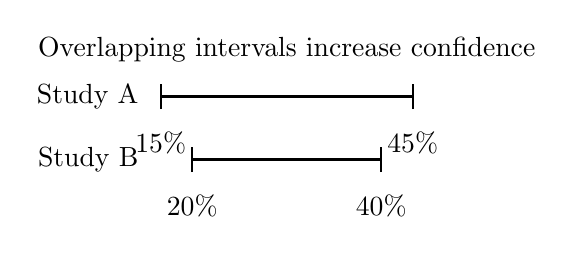
\begin{tikzpicture}[scale=0.8]
					% Draw confidence intervals for two studies
					\draw[thick] (1,3) -- (5,3);
					\draw[thick] (1,2.8) -- (1,3.2);
					\draw[thick] (5,2.8) -- (5,3.2);
					\node[left] at (0.8,3) {Study A};
					\node[below] at (1,2.6) {15\%};
					\node[below] at (5,2.6) {45\%};
					
					\draw[thick] (1.5,2) -- (4.5,2);
					\draw[thick] (1.5,1.8) -- (1.5,2.2);
					\draw[thick] (4.5,1.8) -- (4.5,2.2);
					\node[left] at (0.8,2) {Study B};
					\node[below] at (1.5,1.6) {20\%};
					\node[below] at (4.5,1.6) {40\%};
					
					\node[above] at (3,3.4) {Overlapping intervals increase confidence};
				\end{tikzpicture}
			\end{center}
			
		\end{frame}
		
	% Slide 24: Reading Study Results Like a Detective
	\begin{frame}
		\frametitle{Reading Study Results Like a Detective}
		
		\begin{itemize}
			\item Good detective work means asking questions about who conducted the study, who funded it, and whether the researchers had conflicts of interest.
			\item Look for the actual methods used—was this a controlled experiment, an observational study, or a survey?
			\item Check the population studied and consider whether the results apply to people like you or the situation you're interested in.
			\item Compare results across multiple studies to see if there's a consistent pattern or if this study is an outlier.
			\end{itemize}
				
			\begin{alertblock}{Red Flags to Watch For}
				\begin{itemize}
					\item Study funded by a company that benefits from positive results
					\item Very small sample size for the type of claim being made
					\item Results that contradict a large body of previous research
					\item Researchers refusing to share their data or methods
					\item Media headlines that overstate what the study actually found
					\end{itemize}
					\end{alertblock}
					
	\end{frame}
	
	% Slides 25-28: Diverse Studies and Informal Reasoning
	
	% Slide 25: Why Different Studies Give Different Results
	\begin{frame}
		\frametitle{Why Different Studies Give Different Results}
		
		\begin{itemize}
			\item Even well-conducted studies will show different results due to \textbf{sampling variation}—the natural randomness in who gets selected.
			\item Different research teams may use different methods for measuring the same thing or defining key terms.
			\item The populations studied may differ in important ways—a study of college students may not apply to elderly adults.
			\item Timing and context matter enormously, as social attitudes, health behaviors, and economic conditions change over time.
		\end{itemize}
		
		\begin{exampleblock}{Example}
			Three studies examine whether homework improves student performance. Study A (suburban schools) shows large benefits, Study B (urban schools) shows small benefits, and Study C (rural schools) shows no benefits. These differences might reflect real variation in how homework works in different contexts, not flaws in the research.
		\end{exampleblock}
		
	\end{frame}
	
	% Slide 26: Biased Questions in Consumer Research
	\begin{frame}
		\frametitle{Biased Questions in Consumer Research}
		
		\begin{itemize}
			\item Companies often conduct surveys about their products, but the question wording can strongly influence responses.
			\item \textbf{Leading questions} steer respondents toward the answer the company wants to hear.
			\item The order of questions can also bias results—asking about quality before asking about price makes people more price-sensitive.
			\item Legitimate market research uses neutral wording and follows ethical guidelines to get honest customer feedback.
		\end{itemize}
		
		\begin{alertblock}{Examples of Biased vs. Fair Questions}
			\begin{itemize}
				\item Bad: "How much do you love our amazing new smartphone?"
				\item Better: "How would you rate your satisfaction with this smartphone?"
				\item Bad: "Would you pay extra for our premium quality service?"
				\item Better: "Would you be willing to pay \$5 more per month for faster service?"
			\end{itemize}
		\end{alertblock}
		
	\end{frame}
	
	% Slide 27: Informal Reasoning About Patterns
	\begin{frame}
		\frametitle{Informal Reasoning About Patterns}
		
		\begin{itemize}
			\item We constantly make informal statistical inferences: "This coffee shop is usually crowded" or "My car is reliable."
			\item These judgments involve the same logic as formal studies—we observe a sample of experiences and generalize to future expectations.
			\item The quality of our informal reasoning depends on how representative our experiences are and how much variation we've observed.
			\item Being aware of this process helps us recognize when our "sample size" is too small to support strong conclusions.
		\end{itemize}
		
		\begin{block}{Everyday Statistical Thinking}
			\begin{itemize}
				\item \textbf{Restaurant choice}: "I've had good meals here 4 out of 5 times"
				\item \textbf{Route planning}: "The highway is faster than side streets most mornings"
				\item \textbf{Product reviews}: "Three friends recommended this brand"
				\item \textbf{Weather expectations}: "It usually rains in April here"
			\end{itemize}
			Each involves generalizing from limited observations to broader patterns.
		\end{block}
		
	\end{frame}
	
	% Slide 28: When Our Informal Samples Mislead Us
	\begin{frame}
		\frametitle{When Our Informal Samples Mislead Us}
		
		\begin{itemize}
			\item Our personal experiences can be biased samples that don't represent the broader reality we're trying to understand.
			\item We tend to notice and remember dramatic or unusual events more than typical ones, skewing our perception of what's normal.
			\item Our social circles often share similar characteristics, limiting the diversity of experiences we observe.
			\item Recognizing these limitations helps us seek out additional information before making important decisions.
		\end{itemize}
		
		\begin{exampleblock}{Example}
			Sarah concludes that "all teenagers are rude" based on her interactions with her neighbor's teenage son and a few incidents at the mall. Her sample is biased because she notices rude behavior more than polite behavior, and most of her interactions are with one particular teenager. A more systematic approach would seek out diverse interactions or research on teenage behavior patterns.
		\end{exampleblock}
		
	\end{frame}

% Slides 29-32: Common Errors and Pitfalls

% Slide 29: Correlation vs. Causation
\begin{frame}
	\frametitle{Correlation vs. Causation}
	
	\begin{itemize}
		\item \textbf{Correlation} means two things tend to occur together or change together, while \textbf{causation} means one thing actually causes the other.
		\item Just because two variables are correlated doesn't mean one causes the other—there might be a third factor causing both.
		\item This confusion leads to many false claims in media reports about health, education, and social issues.
		\item Establishing causation requires carefully controlled experiments or very strong observational evidence with multiple lines of support.
	\end{itemize}
	
	\begin{example}
		A study in Springfield finds that neighborhoods with more ice cream sales have higher crime rates. Does ice cream cause crime? No! Both ice cream sales and crime rates increase during hot summer months. Temperature is the hidden factor that explains both trends—this is called a \textbf{confounding variable}.
	\end{example}
	
\end{frame}

% Slide 30: The Dangers of Cherry-Picking Data
\begin{frame}
	\frametitle{The Dangers of Cherry-Picking Data}
	
	\begin{itemize}
		\item \textbf{Cherry-picking} involves selecting only the data points that support your preferred conclusion while ignoring contradictory evidence.
		\item This practice destroys the integrity of statistical reasoning because it abandons the principle of considering all relevant evidence.
		\item People often cherry-pick unconsciously by remembering studies that confirm their beliefs and forgetting those that don't.
		\item Good statistical reasoning requires looking at the full picture, including studies that challenge your expectations.
	\end{itemize}
	
	\begin{alertblock}{Cherry-Picking in Action}
		A Gotham City councilman claims that crime is rising, citing statistics from three neighborhoods. However, he ignores that crime fell in 15 other neighborhoods during the same period. By selecting only supportive data, he creates a misleading picture of the city's overall crime trends.
	\end{alertblock}
	
\end{frame}

% Slide 31: Survivorship Bias in Action
\begin{frame}
	\frametitle{Survivorship Bias in Action}
	
	\begin{itemize}
		\item \textbf{Survivorship bias} occurs when we only examine successful cases while ignoring failures, leading to false conclusions about what causes success.
		\item This bias is especially common in business advice, self-help claims, and investment strategies.
		\item We naturally hear more from people who succeeded than from those who failed, skewing our perception of how effective certain strategies really are.
		\item To avoid this bias, we need to actively seek out information about failures and unsuccessful attempts.
	\end{itemize}
	
	\begin{example}
		The Emerald City Business Journal profiles 10 entrepreneurs who dropped out of college and became millionaires. The article concludes that dropping out leads to business success. This ignores the thousands of college dropouts who failed in business and aren't featured in success stories. The survivors get all the attention while the failures remain invisible.
		\end{example}
			
		\end{frame}
		
		% Slide 32: The Fallacy of Hasty Generalization
		\begin{frame}
			\frametitle{The Fallacy of Hasty Generalization}
			
			\begin{itemize}
				\item A \textbf{hasty generalization} occurs when we draw broad conclusions from too few examples or from unrepresentative cases.
				\item This fallacy is especially tempting when the examples are vivid, recent, or personally meaningful to us.
				\item Our brains are wired to see patterns even in small amounts of data, but this can lead us astray in statistical reasoning.
				\item Good statistical thinking requires resisting the urge to generalize until we have adequate evidence from proper sampling.
			\end{itemize}
			
			\begin{block}{Examples of Hasty Generalization}
				\scriptsize
				\begin{itemize}
					\item "I know three people who got sick after the flu shot, so vaccines are dangerous"
					\item "My neighbor's electric car broke down twice, so electric cars are unreliable"
					\item "The last two Springfield mayors were corrupt, so all politicians are corrupt"
					\item "It snowed in May, so global warming isn't real"
				\end{itemize}
				Each conclusion jumps from limited examples to sweeping claims about entire categories.
			\end{block}
			
		\end{frame}
		
		% Slides 33-36: Common Errors and Conclusion
		
		% Slide 33: When Anecdotes Override Statistics
		\begin{frame}
			\frametitle{When Anecdotes Override Statistics}
			
			\begin{itemize}
				\item An \textbf{anecdote} is a single story or personal experience, while statistics represent patterns across many cases.
				\item Anecdotes are powerful and memorable, but they can mislead us about what's typical or likely to happen.
				\item Our brains give too much weight to vivid stories compared to abstract numbers, even when the numbers are based on much better evidence.
				\item Good statistical reasoning means appreciating both individual stories and broader patterns while recognizing the limitations of each.
			\end{itemize}
			
			\begin{example}
				Springfield's local news features a story about someone who won \$50,000 playing the lottery after buying tickets every day for 20 years. The story is inspiring but doesn't mention the thousands of people who spent similar amounts and won nothing. The anecdote makes lottery playing seem more promising than the statistical reality of extremely low odds.
				\end{example}
					
				\end{frame}
				
				% Slide 34: Becoming a Critical Consumer of Statistics
				\begin{frame}
					\frametitle{Becoming a Critical Consumer of Statistics}
					
					\begin{itemize}
						\item A critical consumer asks probing questions about any statistical claim before accepting it as reliable evidence.
						\item You don't need to be a mathematician to evaluate statistical arguments—focus on the logic and methodology behind the numbers.
						\item Healthy skepticism doesn't mean rejecting all statistics, but rather developing the skills to distinguish good evidence from poor evidence.
						\item These skills help you make better decisions in all areas of life, from health choices to financial investments to voting.
					\end{itemize}
					
					\begin{block}{The Critical Consumer's Mindset}
						\begin{itemize}
							\item \textbf{Curious}: What story do these numbers really tell?
							\item \textbf{Skeptical}: What could be wrong with this study?
							\item \textbf{Contextual}: How does this fit with other evidence?
							\item \textbf{Practical}: What should I do with this information?
						\end{itemize}
					\end{block}
					
				\end{frame}
				
				% Slide 35: Questions to Ask About Any Study or Poll
				\begin{frame}
					\frametitle{Questions to Ask About Any Study or Poll}
					
					\begin{itemize}
						\item Always ask about the sample: Who was included, how were they chosen, and how many people participated?
						\item Question the timing and context: When was this conducted, and what events might have influenced the results?
						\item Examine the questions or measurements: What exactly was asked, and could the wording have biased responses?
						\item Consider the source: Who conducted and funded the study, and what might their motivations be?
					\end{itemize}
					
					\begin{alertblock}{Your Statistical Checklist}
						\begin{enumerate}
							\item Is the sample representative of the population of interest?
							\item Is the sample size adequate for the claims being made?
							\item Could there be sampling bias or non-response bias?
							\item Are the questions fair and unbiased?
							\item Who benefits if people believe these results?
							\item Do these results fit with other reliable evidence?
						\end{enumerate}
					\end{alertblock}
					
				\end{frame}
				
				% Slide 36: Statistical Reasoning: Your Toolkit for Life
				\begin{frame}
					\frametitle{Statistical Reasoning: Your Toolkit for Life}
					
					\begin{itemize}
						\item Statistical reasoning is a powerful form of inductive thinking that helps us learn about the world from limited information.
						\item These skills protect you from being misled by biased surveys, cherry-picked data, and misleading claims in media and advertising.
						\item Good statistical thinking combines healthy skepticism with openness to evidence, helping you update your beliefs when presented with reliable data.
						\item Remember: the goal isn't to become a statistics expert, but to think more clearly about evidence and probability in everyday life.
					\end{itemize}
					
					\begin{center}
						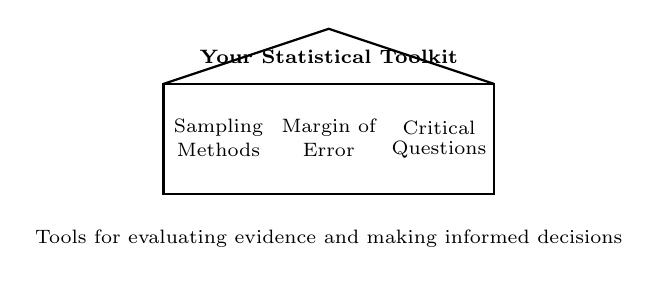
\begin{tikzpicture}[scale=0.7]
							\scriptsize
							% Draw a toolkit
							\draw[thick] (0,0) rectangle (6,2);
							\draw[thick] (0,2) -- (3,3) -- (6,2);
							\node at (3,2.5) {\textbf{Your Statistical Toolkit}};
							
							% Add tools
							\node at (1,1.2) {Sampling};
							\node at (1,0.8) {Methods};
							
							\node at (3,1.2) {Margin of};
							\node at (3,0.8) {Error};
							
							\node at (5,1.2) {Critical};
							\node at (5,0.8) {Questions};
							
							\node[below] at (3,-0.5) {Tools for evaluating evidence and making informed decisions};
						\end{tikzpicture}
					\end{center}
					
				\end{frame}
				
		
\end{document}